\documentclass[12pt,compact]{article}
% \documentclass[main.tex]{subfiles}
\usepackage{amsmath}
\usepackage[normalem]{ulem} % for \sout
\usepackage{graphicx}
\RequirePackage{amsthm,amsmath,multirow,amsfonts,bbm,amssymb,xcolor}
\usepackage{mathtools}  % must be loaded before \DeclarePairedDelimiter
\usepackage[compress]{natbib}
\usepackage{url}

\PassOptionsToPackage{unicode}{hyperref}
\PassOptionsToPackage{hyphens}{url}
\PassOptionsToPackage{dvipsnames,svgnames,x11names}{xcolor}

\usepackage{iftex}
\ifPDFTeX
  \usepackage[T1]{fontenc}
  \usepackage[utf8]{inputenc}
  \usepackage{textcomp} % provide euro and other symbols
\else % if luatex or xetex
  \usepackage{unicode-math}
  \defaultfontfeatures{Scale=MatchLowercase}
  \defaultfontfeatures[\rmfamily]{Ligatures=TeX,Scale=1}
\fi
\usepackage{lmodern}
\ifPDFTeX\else  
    % xetex/luatex font selection
\fi
% Use upquote if available, for straight quotes in verbatim environments
\IfFileExists{upquote.sty}{\usepackage{upquote}}{}
\IfFileExists{microtype.sty}{% use microtype if available
  \usepackage[]{microtype}
  \UseMicrotypeSet[protrusion]{basicmath} % disable protrusion for tt fonts
}{}
\makeatletter
\@ifundefined{KOMAClassName}{% if non-KOMA class
  \IfFileExists{parskip.sty}{%
    \usepackage{parskip} % begin paragraphs with empty line rather than indent
  }{% else
    \setlength{\parindent}{0pt}
    \setlength{\parskip}{6pt plus 2pt minus 1pt}}
}{% if KOMA class
  \KOMAoptions{parskip=half}}
\makeatother
\usepackage{xcolor}
\setlength{\emergencystretch}{3em} % prevent overfull lines
\setcounter{secnumdepth}{5}
% Make \paragraph and \subparagraph free-standing
\makeatletter
\ifx\paragraph\undefined\else
  \let\oldparagraph\paragraph
  \renewcommand{\paragraph}{
    \@ifstar
      \xxxParagraphStar
      \xxxParagraphNoStar
  }
  \newcommand{\xxxParagraphStar}[1]{\oldparagraph*{#1}\mbox{}}
  \newcommand{\xxxParagraphNoStar}[1]{\oldparagraph{#1}\mbox{}}
\fi
\ifx\subparagraph\undefined\else
  \let\oldsubparagraph\subparagraph
  \renewcommand{\subparagraph}{
    \@ifstar
      \xxxSubParagraphStar
      \xxxSubParagraphNoStar
  }
  \newcommand{\xxxSubParagraphStar}[1]{\oldsubparagraph*{#1}\mbox{}}
  \newcommand{\xxxSubParagraphNoStar}[1]{\oldsubparagraph{#1}\mbox{}}
\fi
\makeatother

% NOTE: To produce blinded version, replace "0" with "1" below.
\newcommand{\blind}{0}
\usepackage{rotating}

% DON'T change margins - should be 1 inch all around.
\addtolength{\oddsidemargin}{-.5in}%
\addtolength{\evensidemargin}{-1in}%
\addtolength{\textwidth}{1in}%
\addtolength{\textheight}{1.7in}%
\addtolength{\topmargin}{-1in}%

\newcommand{\red}{\textcolor{red}}

%%%% Non-template packages %%%%
\usepackage{titlesec} % Adjust spacing for sections
\usepackage{tikz}
\usepackage{amsfonts}
\usepackage{natbib} % print author's name and year when citing
\usepackage{bbm}
\usepackage{todonotes}
\usepackage{pdflscape}
\usepackage{caption}
\usepackage{subcaption}
\usepackage{pdfpages}
\usepackage{setspace} 
\usepackage{booktabs}
\usepackage{longtable}
\usepackage{float}
\usepackage{tikz}
\usepackage[colorlinks=true,citecolor=blue, linkcolor=blue]{hyperref}
\usepackage{multirow}
\usepackage{algorithm}
\usepackage{algpseudocode}
\usepackage[defaultlines=2,all]{nowidow} % prevent widows and orphans
\usepackage{enumitem} % inline enumeration
\usepackage{xr-hyper}   % for cross-references that work with hyperref

% penalties for breaking equations
\relpenalty=10000
\binoppenalty=10000

\renewcommand{\theequation}{S.\arabic{equation}}
\renewcommand{\thefigure}{S\arabic{figure}}
\renewcommand{\thesection}{S\arabic{section}}

% Define a custom note command for general notes
\newcommand{\mynote}[1]{\todo[color=yellow!40,inline]{#1}}

% Define custom maths equations 
\DeclareMathOperator{\KL}{KL}
\DeclareMathOperator{\JS}{JS}
\DeclareMathOperator*{\argmin}{arg\,min}
\DeclarePairedDelimiter\abs{\lvert}{\rvert}%
\DeclareMathOperator{\EX}{\mathbb{E}}% expected value
\newcommand{\JSGa}{\mathop{\mathrm{JS}^{\mathrm{G}_{\lambda}}}\nolimits}
\newcommand{\cJSGa}[1]{\mathop{\mathrm{cJS}_{i, #1}^{\mathrm{G}_{\lambda}}}\nolimits}
\newcommand{\eJSGa}[1]{\mathop{\mathrm{eJS}_{i, #1}^{\mathrm{G}_{\lambda}}}\nolimits}
\DeclareRobustCommand{\eJSGai}{\mathop{\mathrm{eJS}^{\mathrm{G}_{\lambda}}}\nolimits}
\DeclareMathOperator{\GJS}{\mathrm{JS}^{\mathrm{G}}}
\DeclareMathOperator{\CE}{\mathrm{CE}}
\newcommand{\rhou}[1]{\rho_{\text{#1}}}
\newcommand\numberthis{\addtocounter{equation}{1}\tag{\theequation}}

\newcommand{\mvmean}[1]{\symbf{\alpha}_{\mid i, #1} y + y^{\symbf{\beta}_{\mid i, #1}} \symbf{\mu}_{\mid i, #1}}
\newcommand{\mvcov}[1]{\left(y^{\symbf{\beta}_{\mid i, #1}}\right)^{\mathrm{T}} \Sigma_{\mid i, #1} y^{\symbf{\beta}_{\mid i, #1}}}

% external document for cross-referencing
\externaldocument{paper}

\begin{document}

\def\spacingset#1{\renewcommand{\baselinestretch}%
{#1}\small\normalsize} \spacingset{1}

%%%%%%%%%%%%%%%%%%%%%%%%%%%%%%%%%%%%%%%%%%%%%%%%%%%%%%%%%%%%%%%%%%%%%%%%%%%%%%

\if0\blind
{
  % \title{\bf Supplementary material for ``Clustering of multivariate tail dependence using conditional methods''}
  \title{\bf Supplementary material for ``???''}
  \author{
  Patrick O'Toole\thanks{Patrick O'Toole is supported by a scholarship from the EPSRC Centre for Doctoral Training in Statistical Applied Mathematics at Bath (SAMBa), under the project EP/S022945/1.}\\
  Department of Mathematical Sciences, University of Bath, UK
  \and
  Christian Rohrbeck\\
  Department of Mathematical Sciences, University of Bath, UK 
  \and
  Jordan Richards\\
  School of Mathematics \\
  and Maxwell Institute for Mathematical Sciences, \\
  University of Edinburgh, UK
  }
  \maketitle
} \fi

\if1\blind
{
  \bigskip
  \begin{center}
    {\LARGE\bf Title}
\end{center}
  \medskip
} \fi

\begin{abstract}
  This supplementary materials contains $\ldots$
\end{abstract}

\newpage
\spacingset{1.75} % DON'T change the spacing!

% --- Tighter spacing around figures and equations ---
\setlength{\textfloatsep}{10pt plus 1pt minus 2pt}
\setlength{\intextsep}{8pt plus 1pt minus 2pt}
\setlength{\floatsep}{8pt plus 1pt minus 2pt}

\setlength{\abovedisplayskip}{8pt plus 2pt minus 4pt}
\setlength{\belowdisplayskip}{8pt plus 2pt minus 4pt}
\setlength{\abovedisplayshortskip}{4pt plus 2pt minus 4pt}
\setlength{\belowdisplayshortskip}{4pt plus 2pt minus 4pt}

\section{Global type I error rate for simulation changepoint detection}

\section{Clustering solution for Spring}

\begin{figure}[htb]
\centering
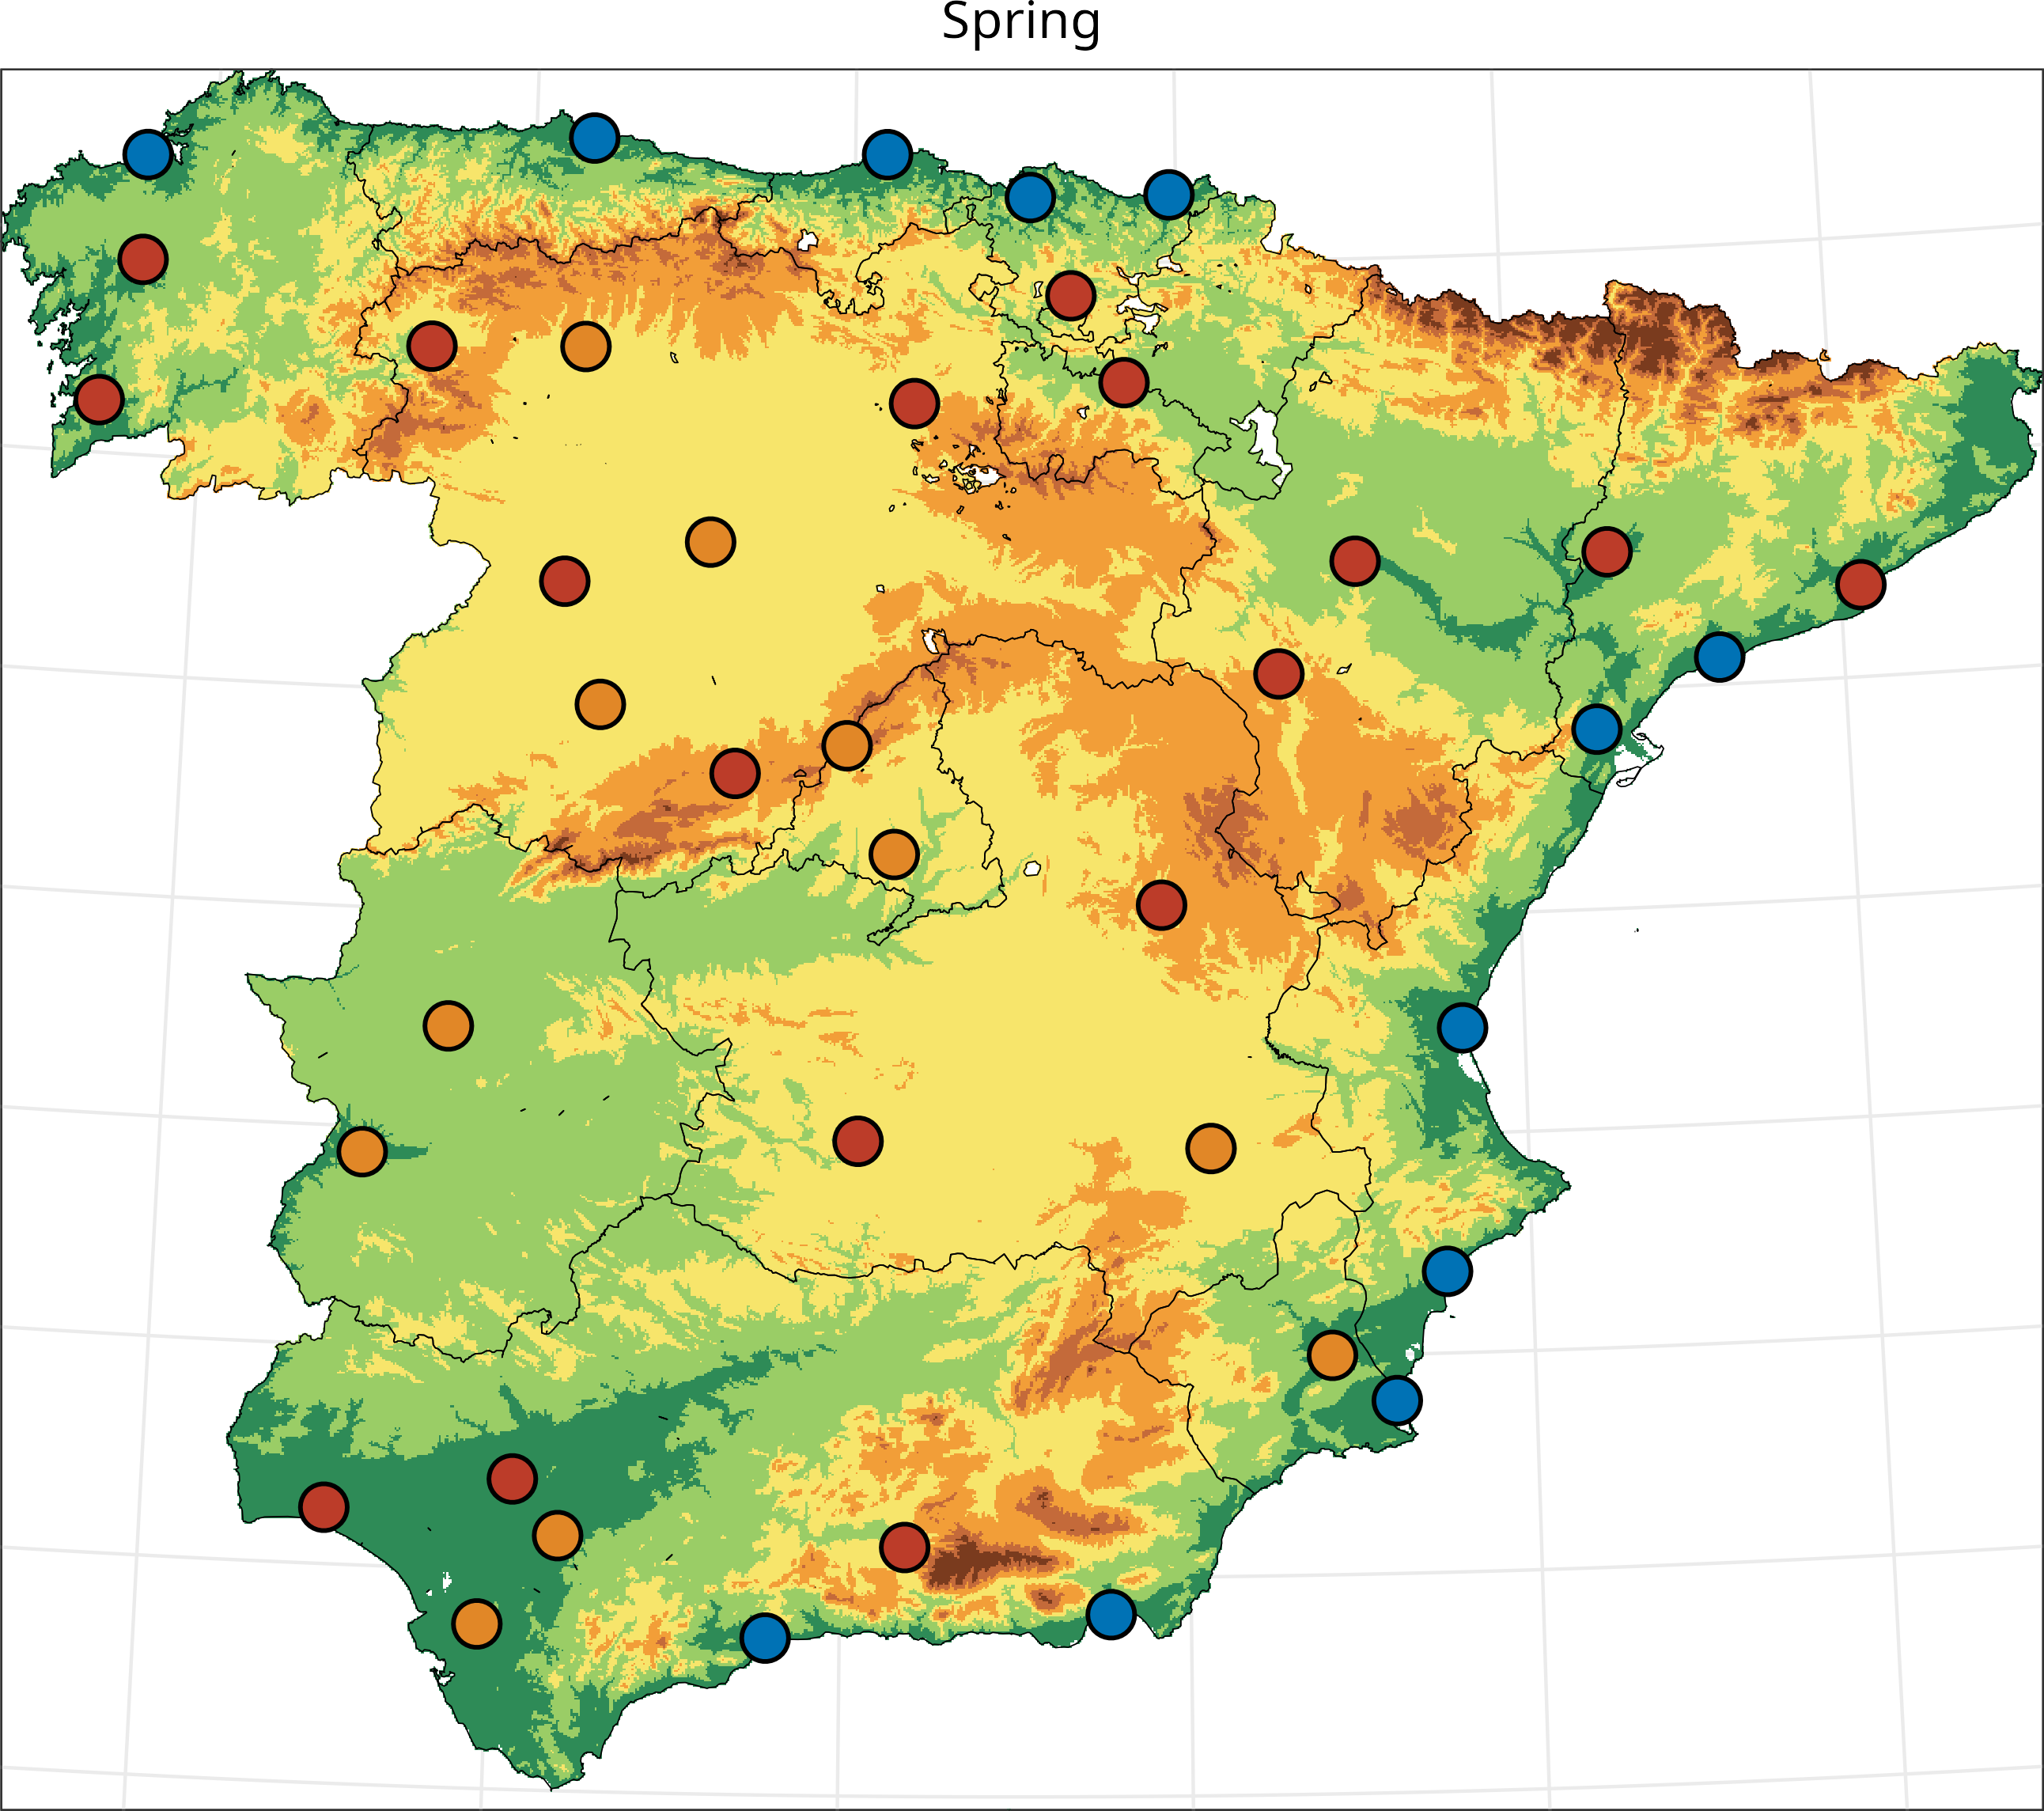
\includegraphics[width=0.9\linewidth]{plots/clust_map_dqu_0.8_spring_trim.png}
\caption{
Spatial clustering of the 40 Spanish stations obtained from the fitted conditional extremes dissimilarity matrix for spring, using the complete time siries.
Three clusters are used in each fit. 
Colours distinguish cluster membership within each panel.
Background shading represents elevation.
}
\label{fig:app_clust_spring}
\end{figure}

\section{Dissimilarity matrices for each season and changepoint division}

\begin{figure}[htb]
\centering
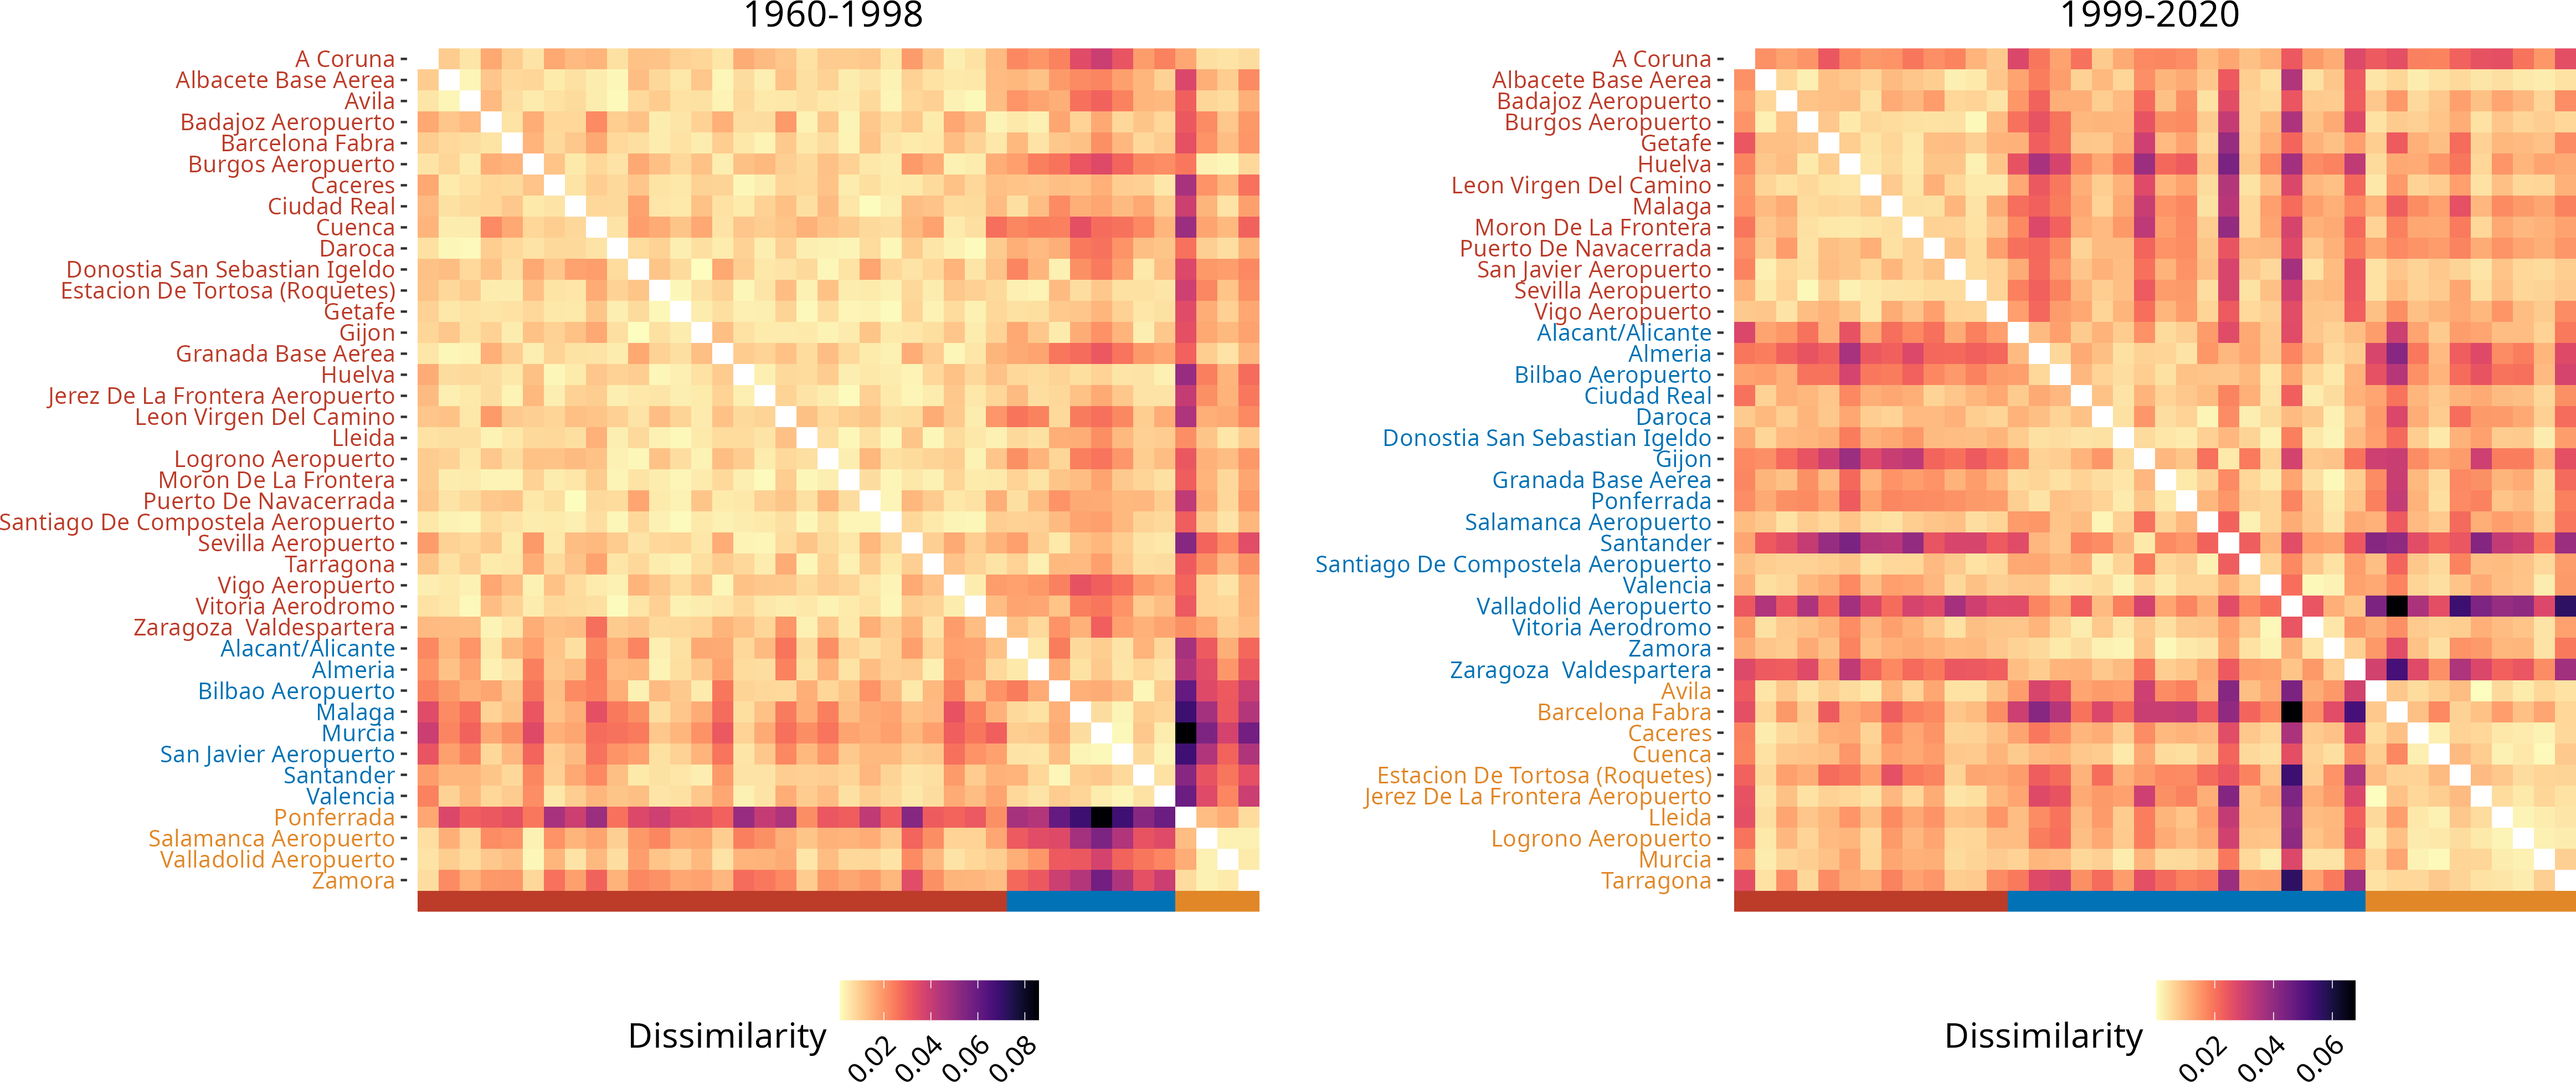
\includegraphics[width=0.9\linewidth]{plots/dist_dqu_0.8_Winter_trim.png}
\caption{
  Aggregated pairwise dissimilarities between the fitted conditional extremes models at the 40 Spanish stations for winter. 
  Results are shown separately for season-years 1960--1998 and 1999--2020. 
  Each matrix entry represents the estimated dissimilarity between the extremal temperature--DPI dependence structures at the corresponding pair of stations. 
  Smaller values indicate more similar fitted dependence structures, while larger values indicate greater dissimilarity. 
  Stations are ordered according to the corresponding three-cluster solution. 
}
\label{fig:diss_winter}
\end{figure}

\begin{figure}[htb]
\centering
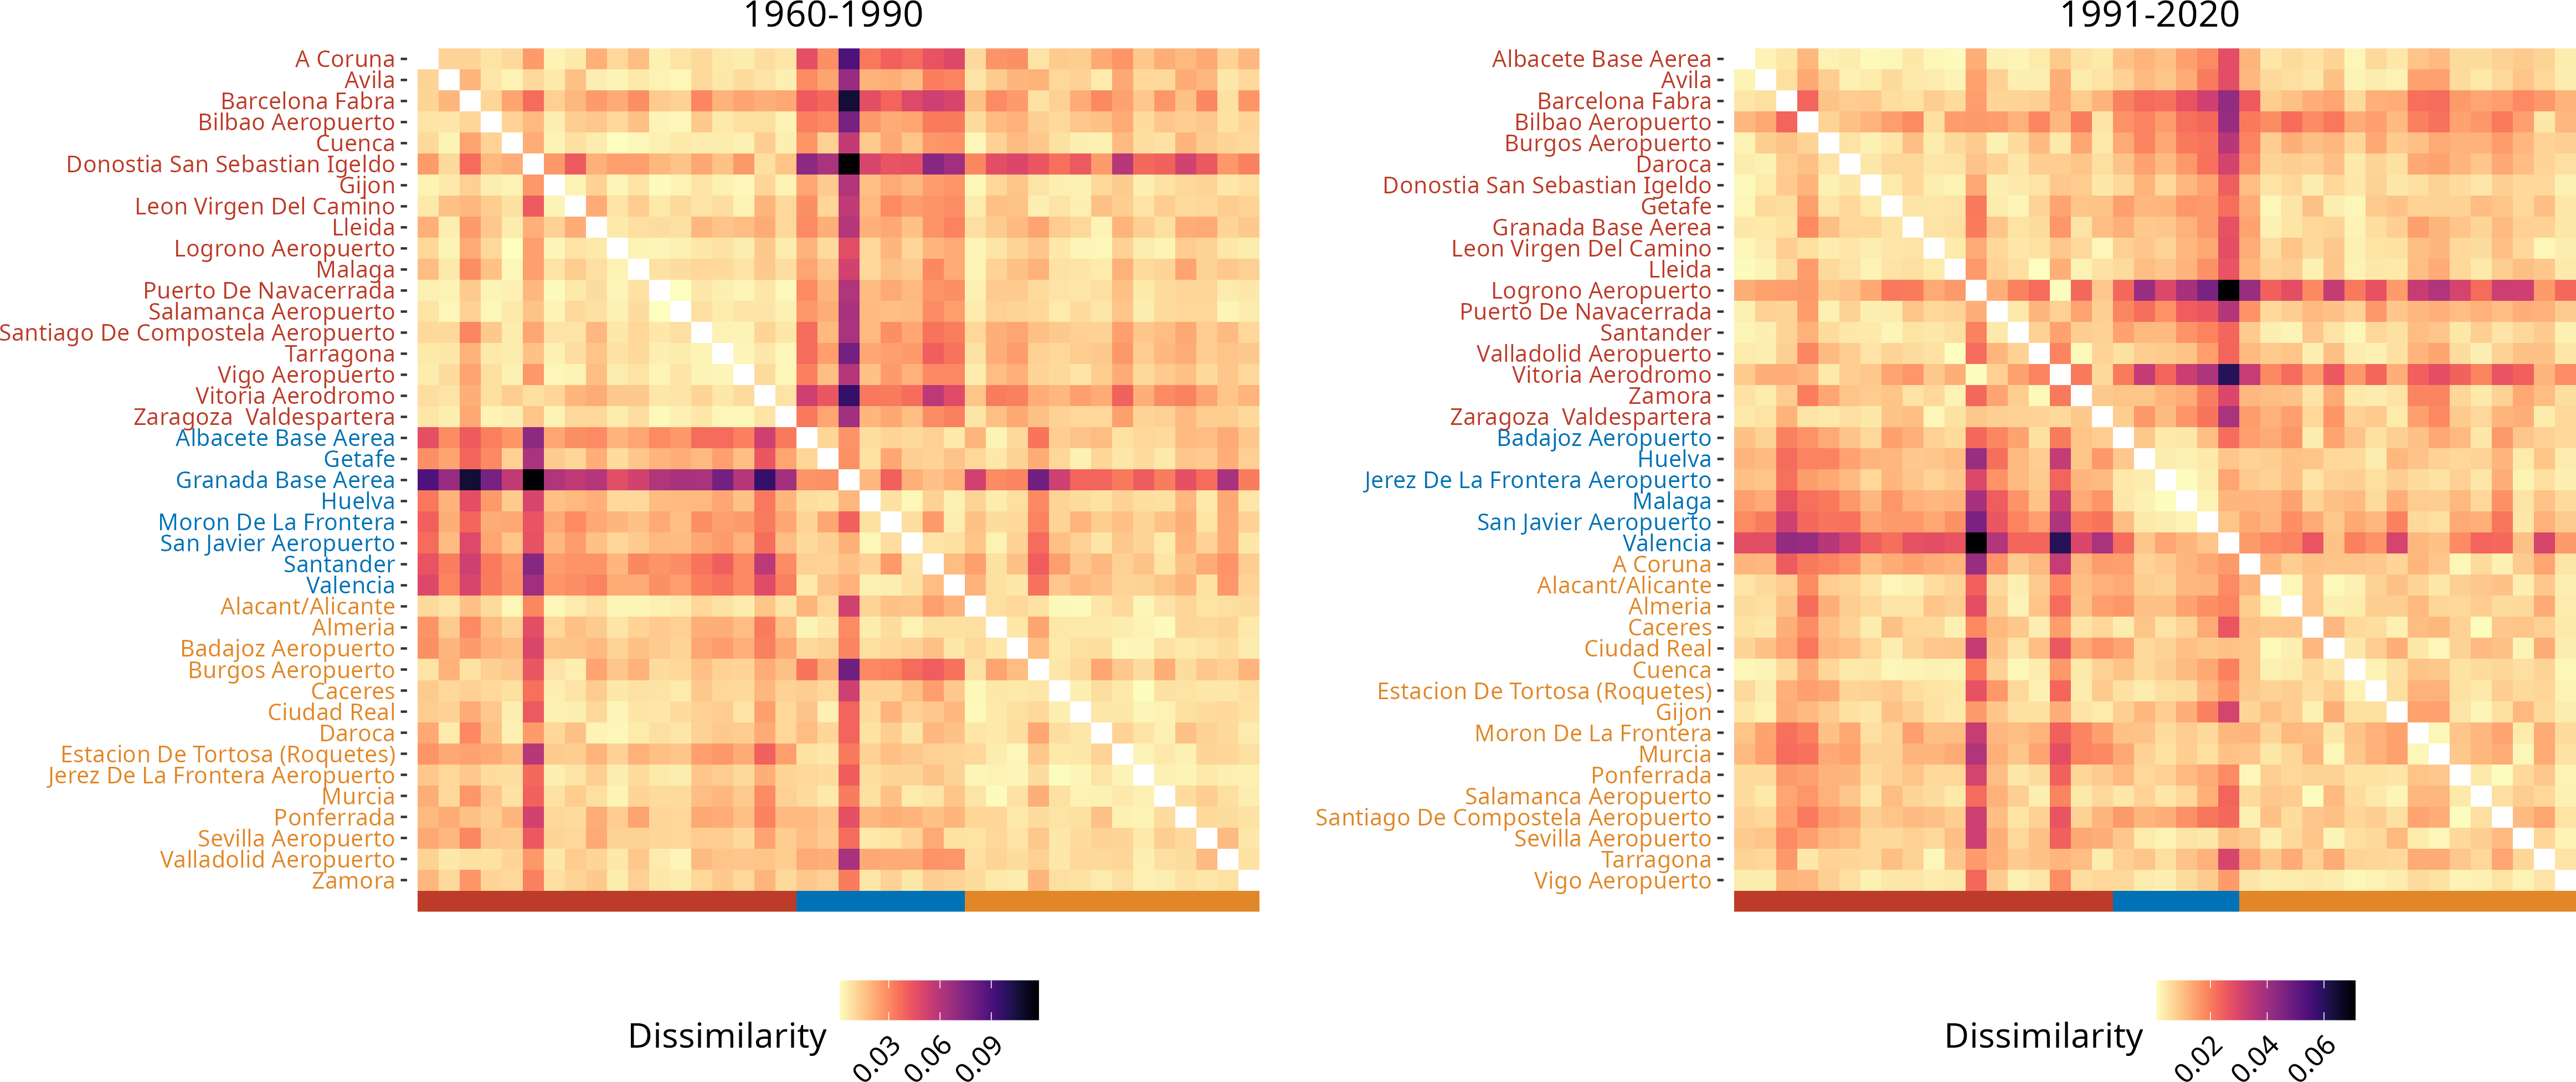
\includegraphics[width=0.9\linewidth]{plots/dist_dqu_0.8_Summer_trim.png}
\caption{
  Aggregated pairwise dissimilarities between the fitted conditional extremes models at the 40 Spanish stations for summer. 
  Results are shown separately for season-years 1960--1990 and 1991--2020. 
  Each matrix entry represents the estimated dissimilarity between the extremal temperature--DPI dependence structures at the corresponding pair of stations. 
  Smaller values indicate more similar fitted dependence structures, while larger values indicate greater dissimilarity. 
  Stations are ordered according to the corresponding three-cluster solution. 
}
\label{fig:diss_summer}
\end{figure}

\begin{figure}[htb]
\centering
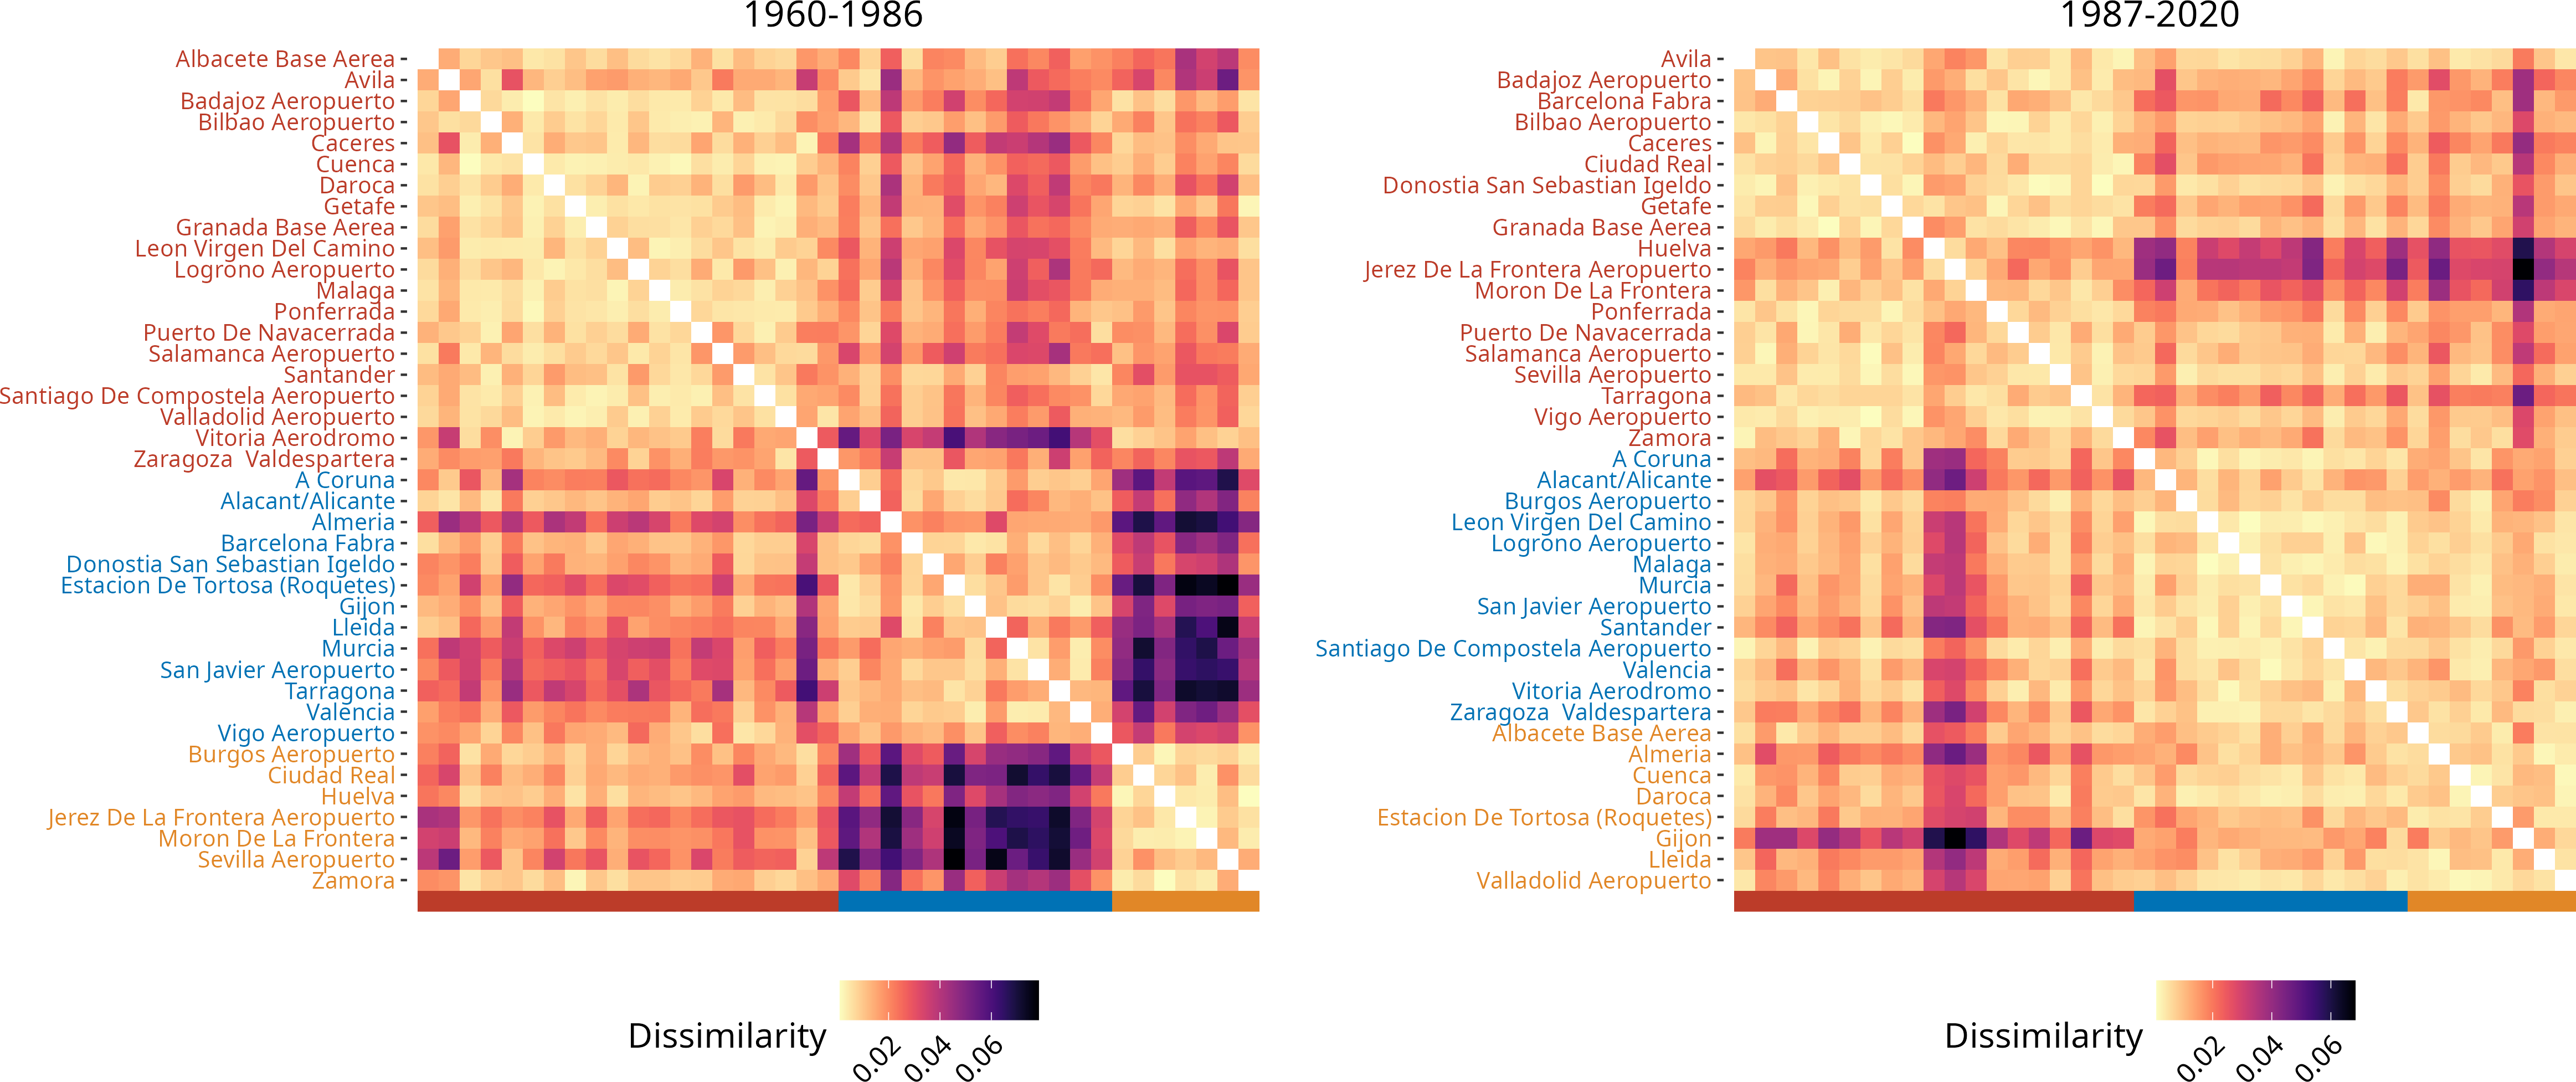
\includegraphics[width=0.9\linewidth]{plots/dist_dqu_0.8_Autumn_trim.png}
\caption{
  Aggregated pairwise dissimilarities between the fitted conditional extremes models at the 40 Spanish stations for autumn. 
  Results are shown separately for season-years 1960--1986 and 1987--2020. 
  Each matrix entry represents the estimated dissimilarity between the extremal temperature--DPI dependence structures at the corresponding pair of stations. 
  Smaller values indicate more similar fitted dependence structures, while larger values indicate greater dissimilarity. 
  Stations are ordered according to the corresponding three-cluster solution. 
}
\label{fig:diss_autumn}
\end{figure}

\begin{figure}[htb]
\centering
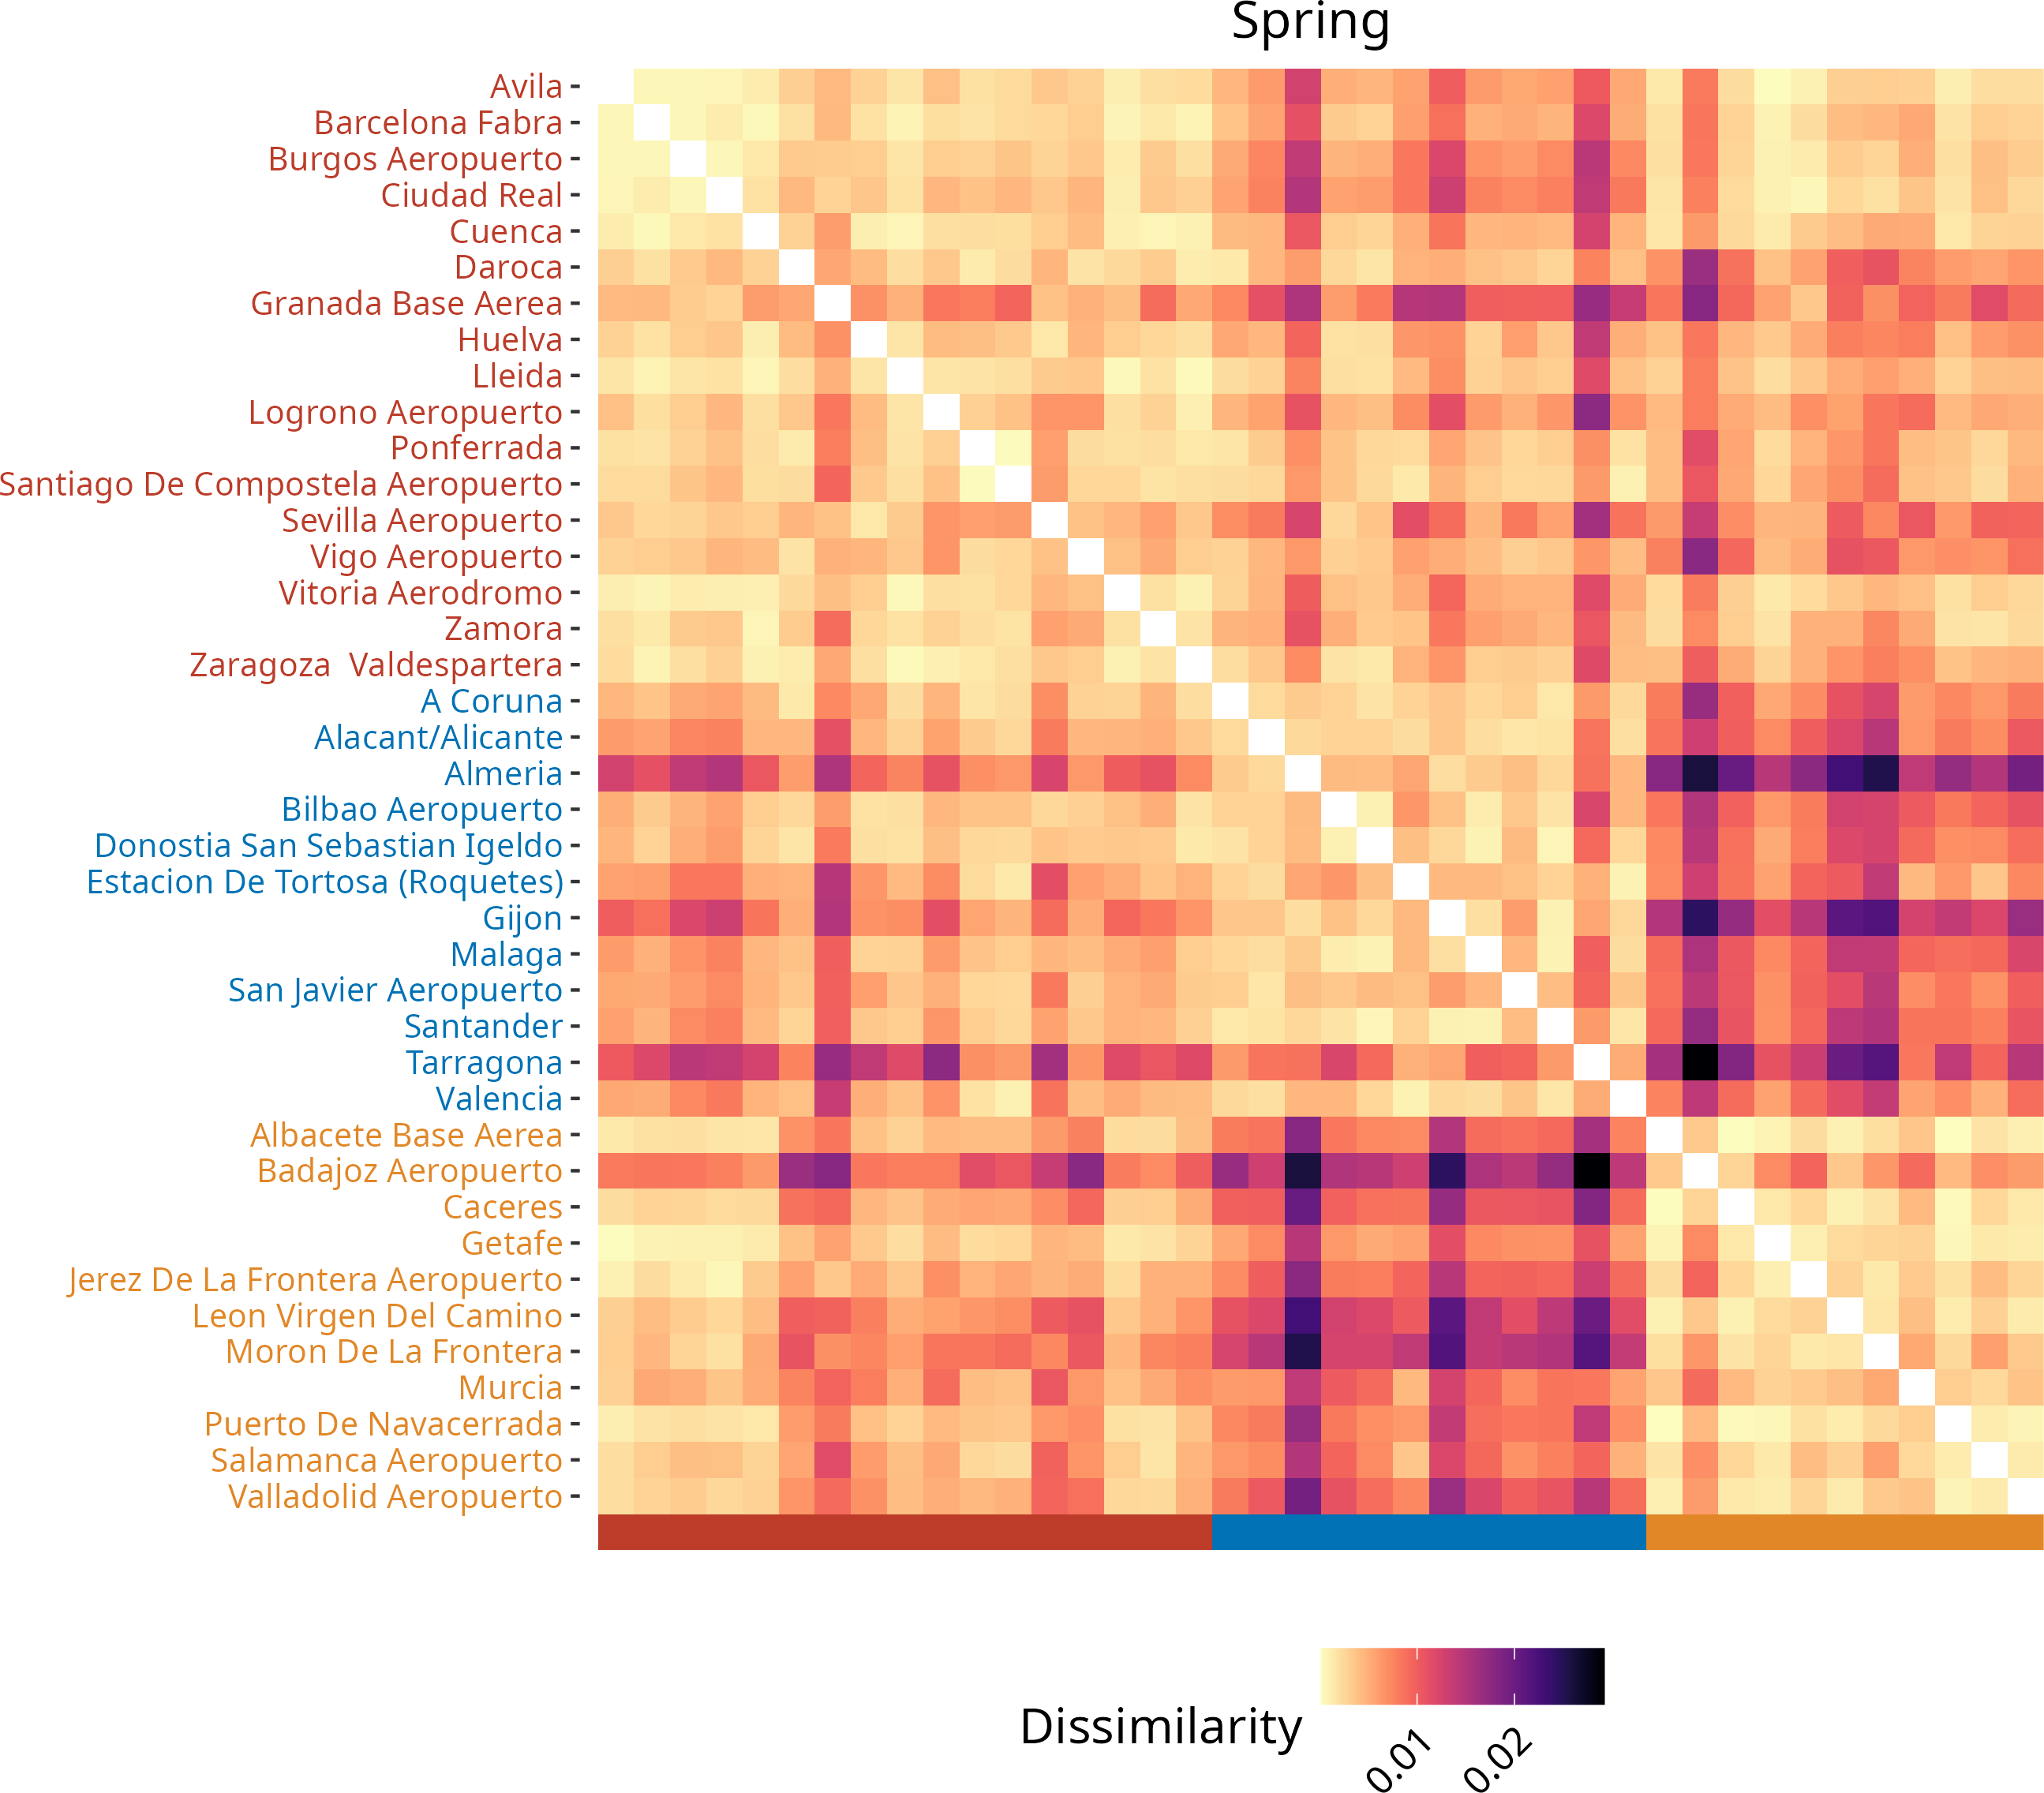
\includegraphics[width=0.9\linewidth]{plots/dist_dqu_0.8_Spring_trim.png}
\caption{
  Aggregated pairwise dissimilarities between the fitted conditional extremes models at the 40 Spanish stations for spring, using the complete time series. 
  Each matrix entry represents the estimated dissimilarity between the extremal temperature--DPI dependence structures at the corresponding pair of stations. 
  Smaller values indicate more similar fitted dependence structures, while larger values indicate greater dissimilarity.
  Stations are ordered according to the three-cluster solution. }
\label{fig:diss_spring}
\end{figure}

\section{Signed matrix differences for each season}

\begin{figure}[htb]
\centering
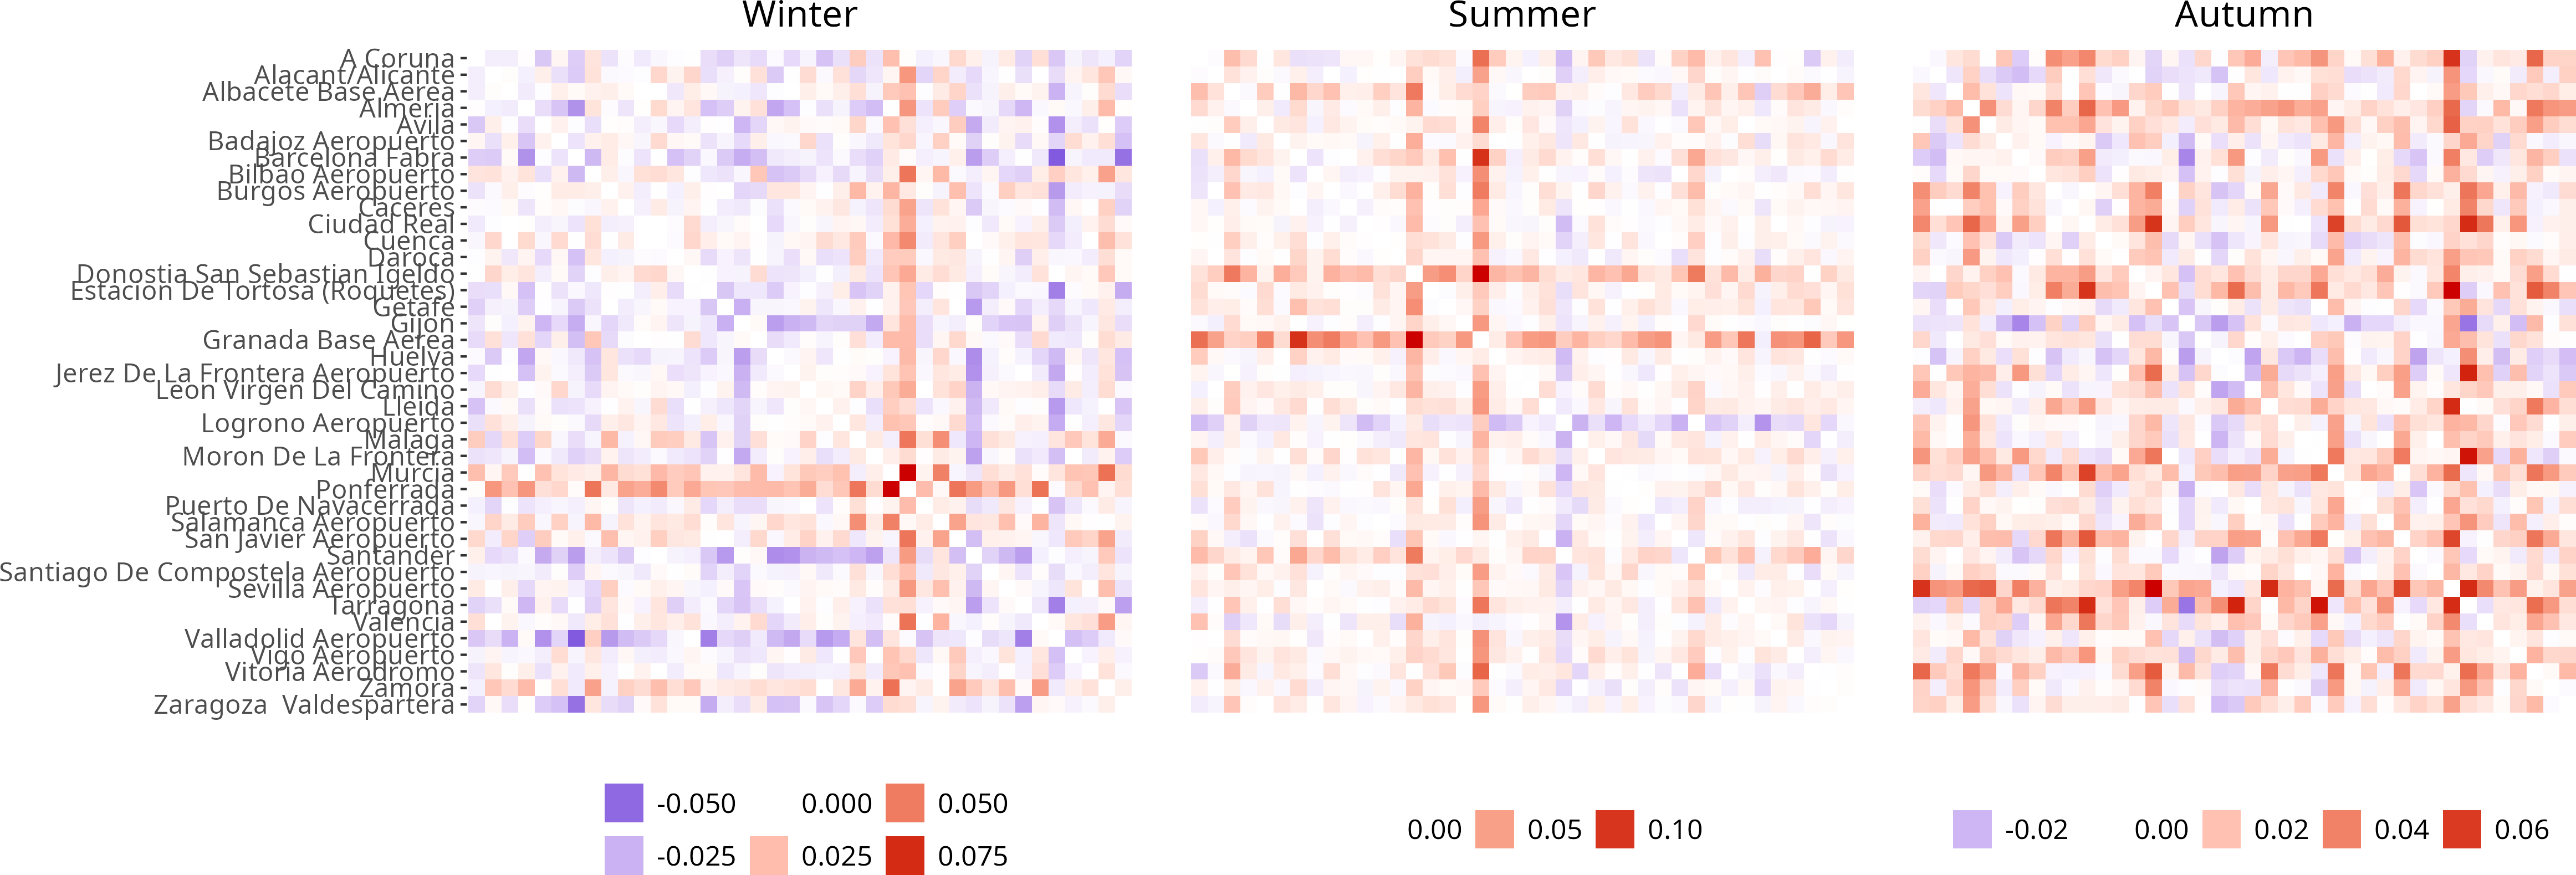
\includegraphics[width=0.9\linewidth]{plots/dist_diff_all_dqu_0.8_trim.png}
\caption{
  Signed changes in the aggregated pairwise dissimilarities between the periods preceding and following the candidate changepoint in each season. 
  Differences are calculated as $D_{\mathrm{before}}-D_{\mathrm{after}}$, using season-years 1960--1998 and 1999--2020 for winter, 1960--1990 and 1991--2020 for summer, and 1960--1986 and 1987--2020 for autumn. 
  Positive entries indicate station pairs that become more similar after the candidate changepoint, whereas negative entries indicate pairs that become more dissimilar. 
  Diagonal entries are zero by construction. 
  Colour scales are defined separately by season and period and their intensities should therefore not be compared directly across panels.
}
\label{fig:sign_matrix_diff}
\end{figure}

\section{Clustering solutions for $k = 2$ and $k = 4$}

\begin{figure}[htb]
\centering
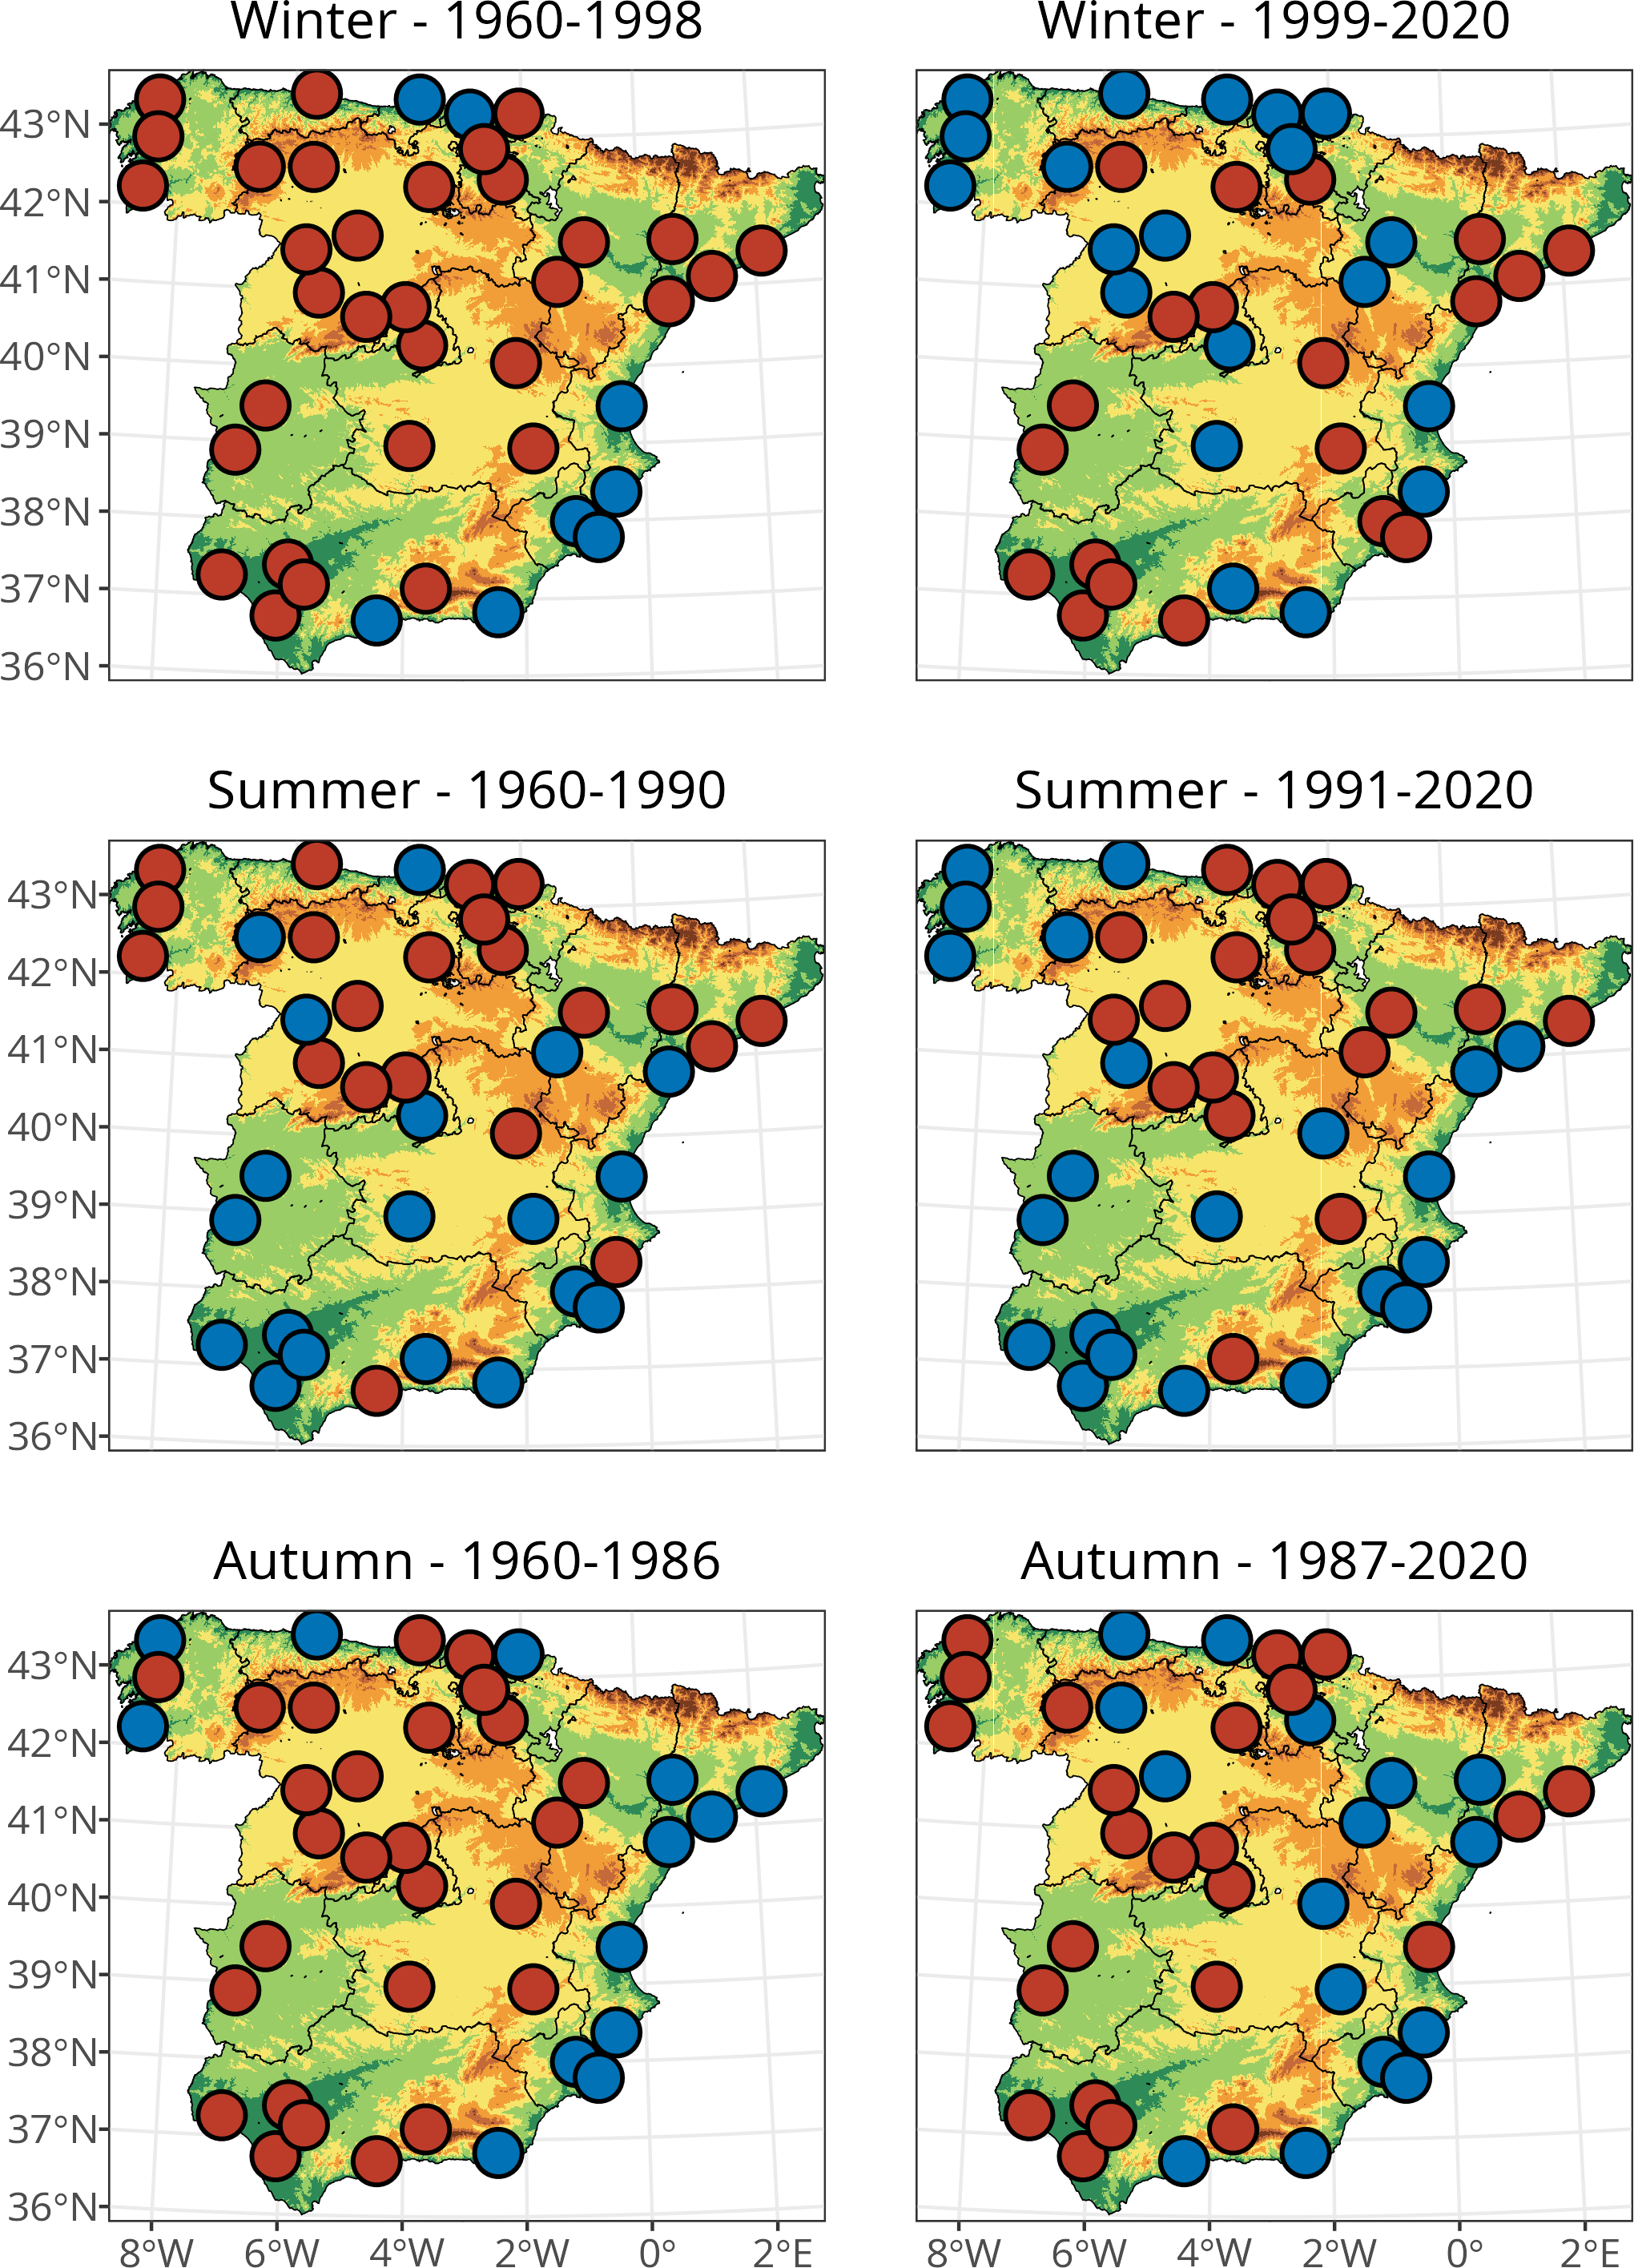
\includegraphics[width=0.9\linewidth]{plots/clust_map_dqu_0.8_k2_trim.png}
\caption{
  Spatial clustering of the 40 Spanish stations obtained from the fitted conditional extremes dissimilarity matrices. 
  Winter is fitted separately for season-years 1960--1998 and 1999--2020, summer for 1960--1990 and 1991--2020, and autumn for 1960--1986 and 1987--2020.
  Two clusters are used in each fit. 
  Colours distinguish cluster membership within each panel.
  Background shading represents elevation.
}
\label{fig:app_clust_k2}
\end{figure}

\begin{figure}[htb]
\centering
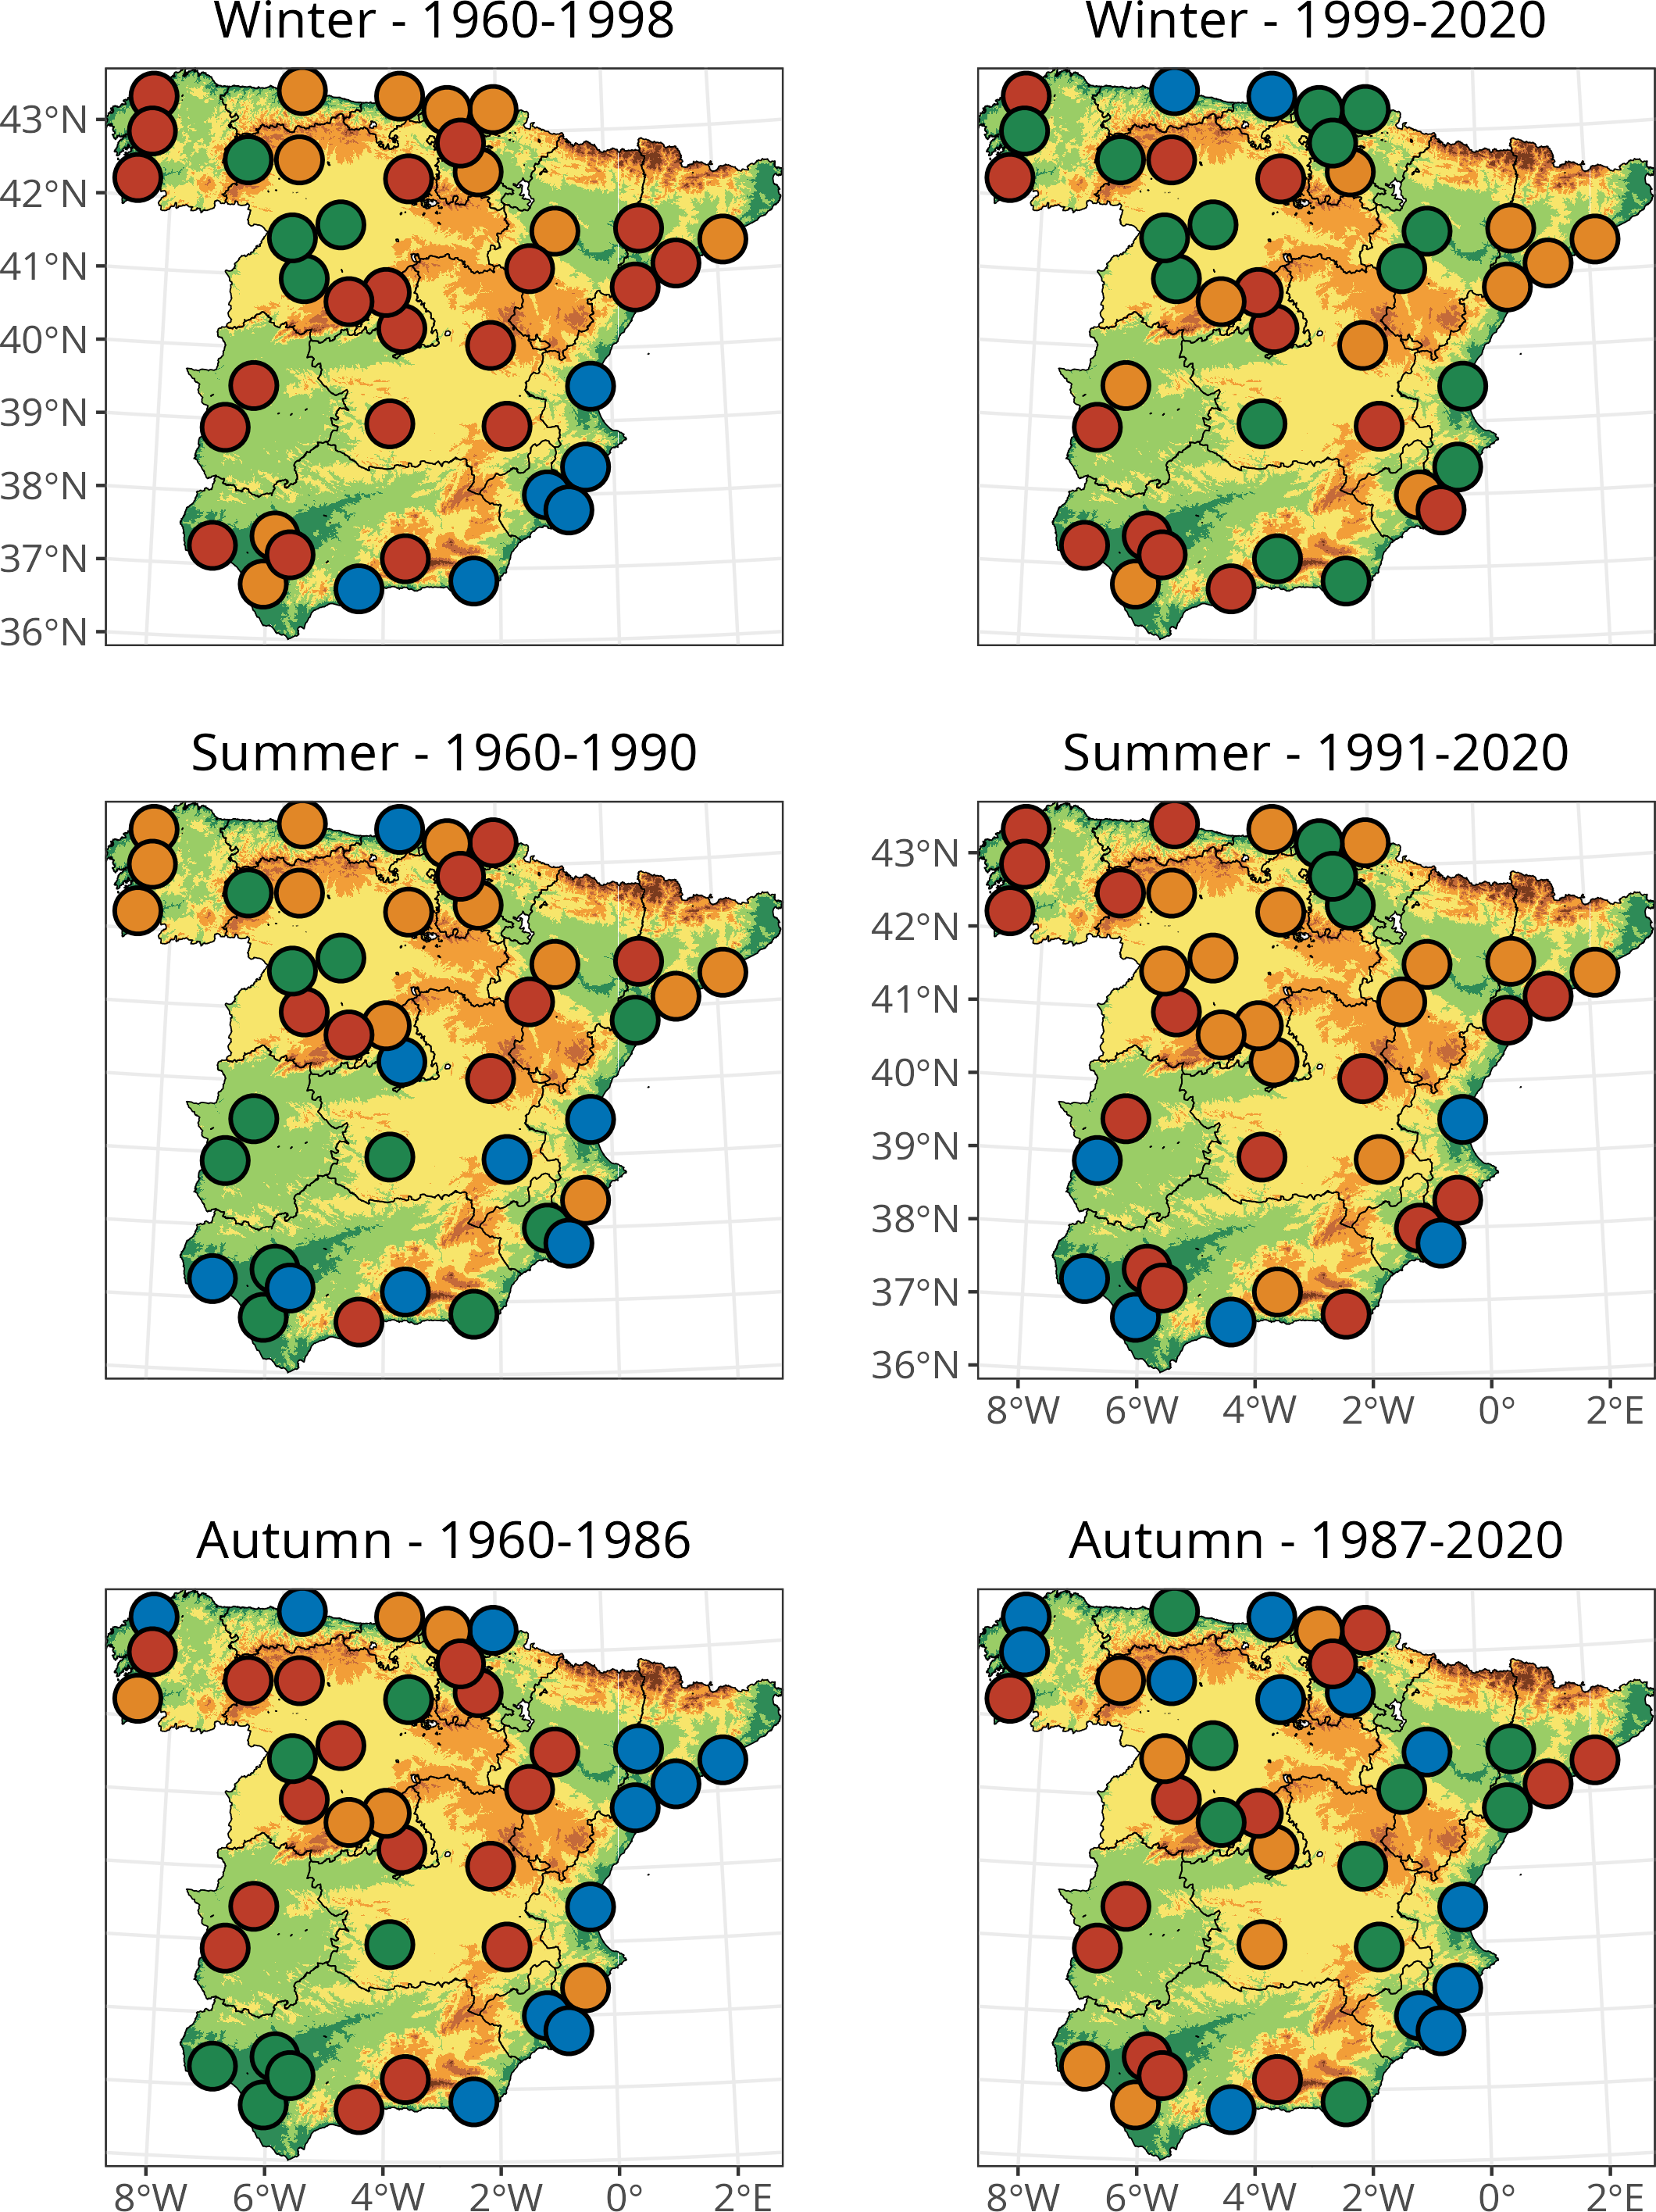
\includegraphics[width=0.9\linewidth]{plots/clust_map_dqu_0.8_k4_trim.png}
\caption{
  Spatial clustering of the 40 Spanish stations obtained from the fitted conditional extremes dissimilarity matrices. 
  Winter is fitted separately for season-years 1960--1998 and 1999--2020, summer for 1960--1990 and 1991--2020, and autumn for 1960--1986 and 1987--2020.
  Four clusters are used in each fit. 
  Colours distinguish cluster membership within each panel.
  Background shading represents elevation.
}
\label{fig:app_clust_k4}
\end{figure}

\begin{figure}[htb]
\centering
\includegraphics[width=0.9\linewidth]{plots/clust_map_k2_k4_spring_trim.png}
\caption{
Spatial clustering of the 40 Spanish stations obtained from the fitted conditional extremes dissimilarity matrices. 
Shown are the clustering solutions for Spring, for the complete time series, for $k = 2$ and $k = 4$ clusters. 
Colours distinguish cluster membership within each panel.
Background shading represents elevation.
}
\label{fig:app_clust_k2_4_spring}
\end{figure}

\bibliographystyle{apalike}
% Don't sort bibliography so it stays in chronological order
{\small
\bibliography{wileyNJD-APA.bib}
}

\end{document}
